\documentclass[border=1cm]{standalone}

\usepackage{charter}

\usepackage{tikz}
\usetikzlibrary{automata, positioning, arrows, decorations.pathreplacing, calc, chains, shapes.misc, backgrounds, fit, patterns, fadings, shadows.blur}

\pgfdeclarelayer{background}
\pgfsetlayers{background, main}

\usepackage{xcolor}

\definecolor{ACMYellow}{RGB}{255, 214, 0}
\definecolor{ACMOrange}{RGB}{252, 146, 0}
\definecolor{ACMRed}{RGB}{253, 27, 20}
\definecolor{ACMLightBlue}{RGB}{131, 206, 226}
\definecolor{ACMGreen}{RGB}{166, 188, 9}
\definecolor{ACMPurple}{RGB}{101, 1, 107}
\definecolor{ACMDarkBlue}{RGB}{9, 53, 122}


\newcommand*\circled[1]{\tikz[baseline=(char.base)]{
            \node[shape=circle, draw, inner sep=2pt, thick] (char) {#1};}}

\begin{document}

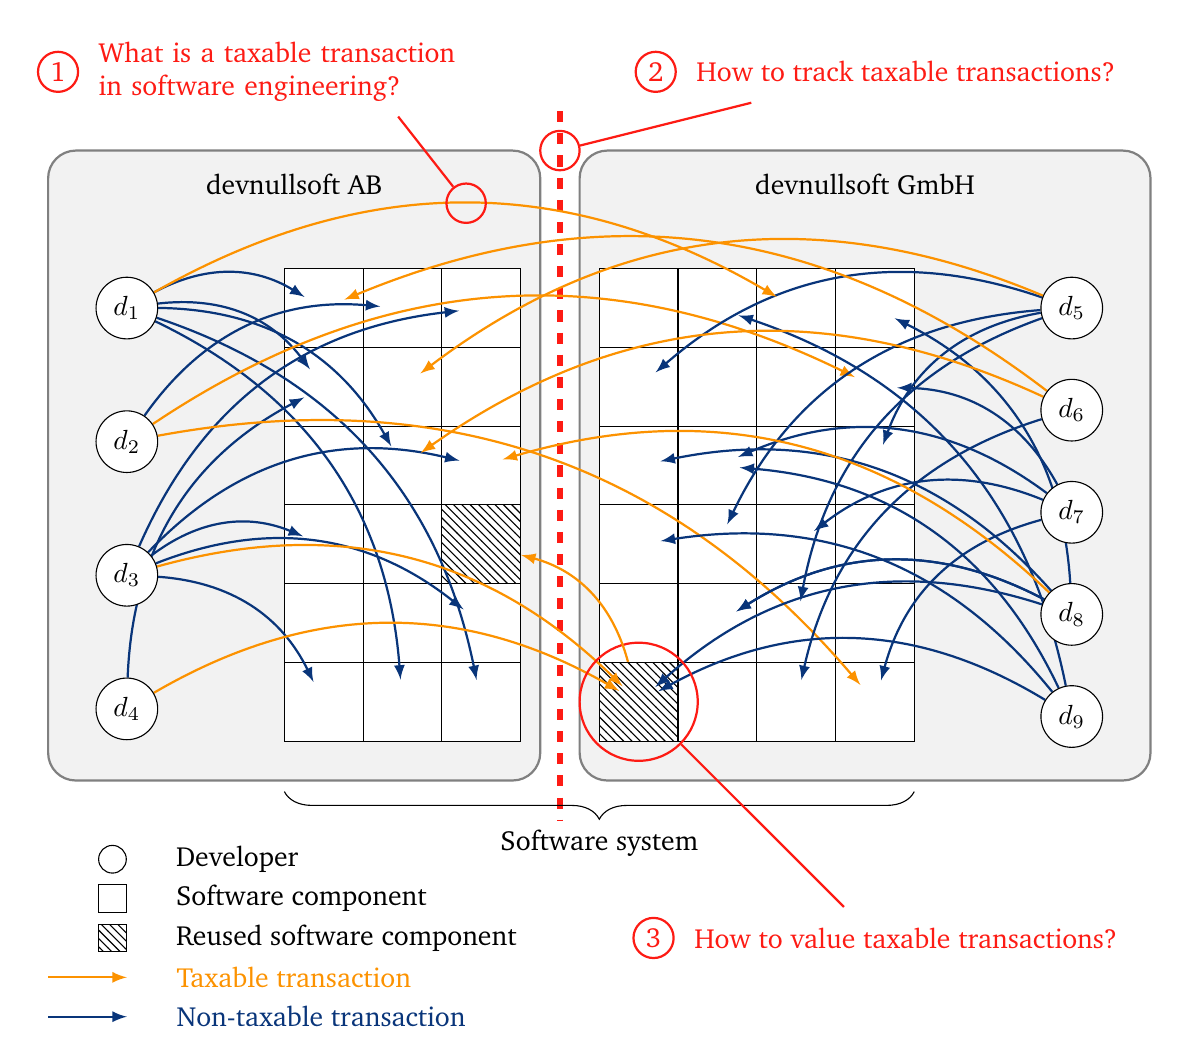
\begin{tikzpicture}

\begin{scope}[xshift=-2cm, start chain=going below, node distance=9mm]
    \foreach \d in {1,2,3,4}
      \node[on chain, draw, circle, fill=white] (d\d) {$d_\d$};
    \end{scope}

    % the vertices of V
    \begin{scope}[xshift=10cm, start chain=going below, node distance=5mm]
    \foreach \d in {5, 6, ..., 9}
      \node[on chain, draw, circle, fill=white] (d\d) {$d_\d$};

\end{scope}


\begin{scope}[yshift=-5.5cm, on background layer]

\node[draw=black!50, thick, rounded corners=1em, fit={(-3, -0.5) (3.25, 7.5)}, rectangle, inner sep=0mm, label={[yshift=-7mm]above:devnullsoft AB}, fill=black!5] (ab) {};
\node[draw=black!50, thick, rounded corners=1em, fit={(3.75, -0.5) (11, 7.5)}, rectangle, inner sep=0mm, label={[yshift=-7mm]above:devnullsoft GmbH}, fill=black!5] (gmbh) {};

\draw[line width=2pt, dash pattern=on 4pt off 4pt, ACMRed] (3.5, 8) -- (3.5, -1);


\draw[fill=white] (0,0) grid (3,6) rectangle (0,0);
\draw[fill=white] (4,0) grid (8,6) rectangle (4,0);

\foreach \x in {0, 1, ..., 7} 
	\foreach \y in {0, 1, ..., 5} {
		\node[circle, shift={(0.5,0.5)}, draw=none, inner sep=2mm, outer sep=0pt] at (\x, \y) (n\x\y) {};
	}

\node[rectangle, minimum size=1cm, pattern=north west lines] (component) at (n22) {};
\node[rectangle, minimum size=1cm, pattern=north west lines] (reusedcomponent) at (n40) {};

\draw[decorate,decoration={brace,amplitude=10pt,mirror,raise=4pt},yshift=0pt]
(0,-0.5) -- (8, -0.5) node [draw=none, midway, yshift=-0.8cm] {Software system};


\foreach \d/\x/\y/\b/\c in {3/2/5/left/ACMDarkBlue, 2/1/5/left/ACMDarkBlue, 1/1/0/left/ACMDarkBlue, 3/2/3/left/ACMDarkBlue, 1/0/5/left/ACMDarkBlue, 1/2/0/left/ACMDarkBlue, 3/0/0/left/ACMDarkBlue, 1/1/3/left/ACMDarkBlue, 3/0/2/left/ACMDarkBlue, 4/0/4/left/ACMDarkBlue, 1/0/4/left/ACMDarkBlue, 3/2/1/left/ACMDarkBlue, 2/7/4/left/ACMOrange, 2/7/0/left/ACMOrange, 5/6/1/right/ACMDarkBlue, 8/4/3/right/ACMDarkBlue, 9/4/2/right/ACMDarkBlue, 7/5/3/right/ACMDarkBlue, 7/7/4/right/ACMDarkBlue, 9/5/5/right/ACMDarkBlue, 9/5/3/right/ACMDarkBlue, 8/7/5/right/ACMDarkBlue, 6/6/0/right/ACMDarkBlue, 8/5/1/right/ACMDarkBlue, 5/4/4/right/ACMDarkBlue, 8/5/1/right/ACMDarkBlue, 7/7/0/right/ACMDarkBlue, 5/5/2/right/ACMDarkBlue, 5/7/3/right/ACMDarkBlue, 7/6/2/right/ACMDarkBlue, 6/0/5/right/ACMOrange, 6/1/3/right/ACMOrange, 5/1/4/right/ACMOrange, 8/2/3/right/ACMOrange, 8/4/0/right/ACMDarkBlue, 3/4/0/left/ACMOrange} \draw[-latex, thick, color=\c] (d\d) to[bend \b] (n\x\y);

\draw[-latex, color=ACMOrange, thick] (d4) to[bend left] (n40);
\draw[-latex, color=ACMDarkBlue, thick] (d9) to[bend right] (n40);

\draw[-latex, color=ACMOrange, thick] (d1) to[bend left] node[midway, circle, draw, ACMRed, minimum size=0.5cm] (transaction) {} (n65);
\node[circle, draw, thick, ACMRed, minimum size=1.5cm] (account) at (n40) {};
\node[circle, draw, thick, ACMRed, minimum size=0.5cm] (tracking) at (3.5, 7.5) {};

\end{scope}


\begin{scope}[xshift=-2cm, yshift=-9cm, y=0.5cm, label distance=5mm]
\node[draw, circle, anchor=east, label=right:Developer, minimum size=1em] at (0,4) {};
\node[draw, rectangle, anchor=east, label=right:Software component, minimum size=1em] at (0,3) {};
\node[draw, rectangle, anchor=east, pattern=north west lines, label=right:Reused software component, minimum size=1em] at (0,2) {};
\draw[-latex, thick, ACMOrange] (-1, 1) -- (0, 1) node[black, label=right:Taxable transaction, anchor=east] {};
\draw[-latex, thick, ACMDarkBlue] (-1, 0) -- (0, 0) node[label=right:Non-taxable transaction, anchor=east] {};
\end{scope}


\draw[ACMOrange, thick, -latex] (reusedcomponent) to[bend right] (component);

\node[ACMRed, every two node part/.style={text width=7.5cm}, align=left, rectangle split, rectangle split horizontal, rectangle split parts=2] (transactiondesc) at (1, 3) {\circled{1}\nodepart{two}What is a taxable transaction\\in software engineering?};
\draw[ACMRed, thick] (transaction) -- (transactiondesc);

\node[ACMRed, align=left, rectangle split, rectangle split horizontal, rectangle split parts=2] (trackingdesc) at (7.5, 3) {\circled{2}\nodepart{two}How to track taxable transactions?};
\draw[ACMRed, thick] (tracking) -- (trackingdesc);


\node[ACMRed, align=left, rectangle split, rectangle split horizontal, rectangle split parts=2] (accountdesc) at (7.5, -8) {\circled{3}\nodepart{two} How to value taxable transactions?};
\draw[ACMRed, thick] (account) -- (accountdesc);


\end{tikzpicture}

\end{document}